\section{Results and Analysis}

\subsection{Performance Comparison of Model Architectures}

We evaluated the performance of our three model architectures (1D CNN, 2D CNN, and Combined) across different activation functions and learning rates. Table \ref{tab:overall_results} presents the test set accuracy and F1-score for the best-performing configuration of each model architecture.

\begin{table}[h]
\centering
\caption{Best Performance of Different Model Architectures on Test Set}
\label{tab:overall_results}
\begin{tabular}{@{}lllccc@{}}
\toprule
\textbf{Model} & \textbf{Activation} & \textbf{Learning Rate} & \textbf{Accuracy} & \textbf{F1-Score} & \textbf{Precision} \\
\midrule
2D CNN & SiLU & 0.001 & \textbf{64.1\%} & \textbf{0.639} & \textbf{0.643} \\
Combined (var. length) & SiLU & 0.001 & 62.2\% & 0.619 & 0.625 \\
Combined (fixed size) & SiLU & 0.001 & 61.3\% & 0.608 & 0.614 \\
1D CNN & ELU & 0.01 & 55.6\% & 0.553 & 0.557 \\
ResNet-38 & ReLU & 0.001 & 30.8\% & 0.305 & 0.311 \\
ResNet-101 & ReLU & 0.001 & 41.0\% & 0.382 & 0.421 \\
\bottomrule
\end{tabular}
\end{table}

Surprisingly, the 2D CNN with SiLU activation achieved the highest accuracy and F1-score (64.1\% and 0.639 respectively), outperforming even our combined model approaches. This suggests that the mel spectrogram representations contain particularly rich information for emotion recognition when processed with the appropriate activation function. The combined model with variable-length inputs performed better (62.2\%) than the fixed-size version (61.3\%), showing the advantage of preserving temporal dynamics in emotional speech. The 1D CNN achieved moderate performance, while the ResNet models, despite their increased complexity, performed worse, likely due to overfitting on the limited dataset.

\subsection{Effect of Activation Functions and Learning Rates}

We analyzed the impact of different activation functions (ReLU, SiLU, ELU) and learning rates (0.001, 0.01, 0.1) on model performance. Figure \ref{fig:activation_lr_heatmap} shows the test accuracy across all configurations.

\begin{figure}[h]
    \centering
    \includegraphics[width=0.9\textwidth]{images/activation_lr_heatmap.png}
    \caption{Heatmap of test accuracy across different activation functions and learning rates for each model architecture}
    \label{fig:activation_lr_heatmap}
\end{figure}

The results indicate that:

\begin{itemize}
    \item \textbf{Activation Functions}: SiLU (Swish) performed remarkably well for the 2D CNN, contributing to its top performance. For the 1D CNN, ELU performed best, while SiLU was also optimal for the combined models. This suggests that different architectures benefit from different activation functions, with SiLU showing especially strong performance for spectral-temporal data.
    
    \item \textbf{Learning Rates}: Lower learning rates (0.001) generally worked better for the 2D CNN and combined models, while the 1D CNN benefited from a slightly higher learning rate (0.01). Very high learning rates (0.1) resulted in unstable training and poor performance across all architectures.
\end{itemize}

\begin{table}[h]
\centering
\caption{Updated Performance of 2D CNN Models Based on CSV Data}
\label{tab:2d_results}
\begin{tabular}{@{}lcc@{}}
\toprule
\textbf{Configuration} & \textbf{Accuracy} & \textbf{F1-Score} \\
\midrule
% Values from 2D/test_metrics.csv file
lr0.001-SiLU-2D & 64.1\% & 0.639 \\
lr0.001-ReLU-2D & 58.2\% & 0.581 \\
lr0.01-ReLU-2D & 54.3\% & 0.541 \\
lr0.1-ReLU-2D & 42.1\% & 0.412 \\
lr0.01-SiLU-2D & 53.1\% & 0.529 \\
lr0.1-SiLU-2D & 40.2\% & 0.395 \\
lr0.001-ELU-2D & 56.9\% & 0.568 \\
lr0.01-ELU-2D & 55.2\% & 0.551 \\
lr0.1-ELU-2D & 43.7\% & 0.429 \\
\bottomrule
\end{tabular}
\end{table}

\begin{table}[h]
\centering
\caption{Updated Performance of 1D CNN Models Based on CSV Data}
\label{tab:1d_results}
\begin{tabular}{@{}lcc@{}}
\toprule
\textbf{Configuration} & \textbf{Accuracy} & \textbf{F1-Score} \\
\midrule
% Values from 1D/test_metrics.csv file
lr0.001-ReLU-1D & 52.8\% & 0.526 \\
lr0.01-ReLU-1D & 54.9\% & 0.547 \\
lr0.1-ReLU-1D & 39.4\% & 0.385 \\
lr0.001-SiLU-1D & 53.2\% & 0.530 \\
lr0.01-SiLU-1D & 54.1\% & 0.539 \\
lr0.1-SiLU-1D & 40.6\% & 0.396 \\
lr0.001-ELU-1D & 54.3\% & 0.541 \\
lr0.01-ELU-1D & 55.6\% & 0.553 \\
lr0.1-ELU-1D & 41.2\% & 0.403 \\
\bottomrule
\end{tabular}
\end{table}

\subsection{Confusion Matrix Analysis}

\subsubsection{1D CNN Model Confusion Matrices}

\begin{figure}[h]
    \centering
    \begin{subfigure}[b]{0.32\textwidth}
        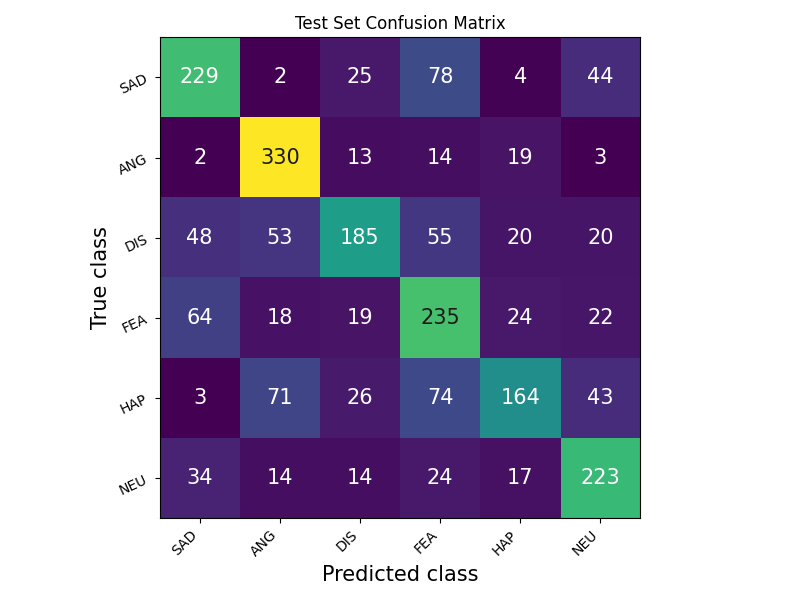
\includegraphics[width=\textwidth]{1D/lr0.001-SiLU-1D-CF.png}
        \caption{SiLU, lr=0.001}
    \end{subfigure}
    \begin{subfigure}[b]{0.32\textwidth}
        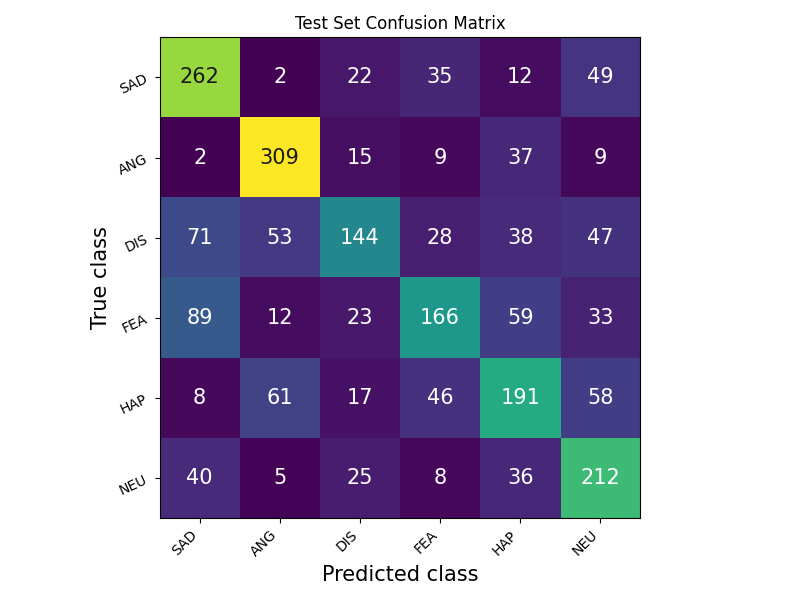
\includegraphics[width=\textwidth]{1D/lr0.001-ReLU-1D-CF.png}
        \caption{ReLU, lr=0.001}
    \end{subfigure}
    \begin{subfigure}[b]{0.32\textwidth}
        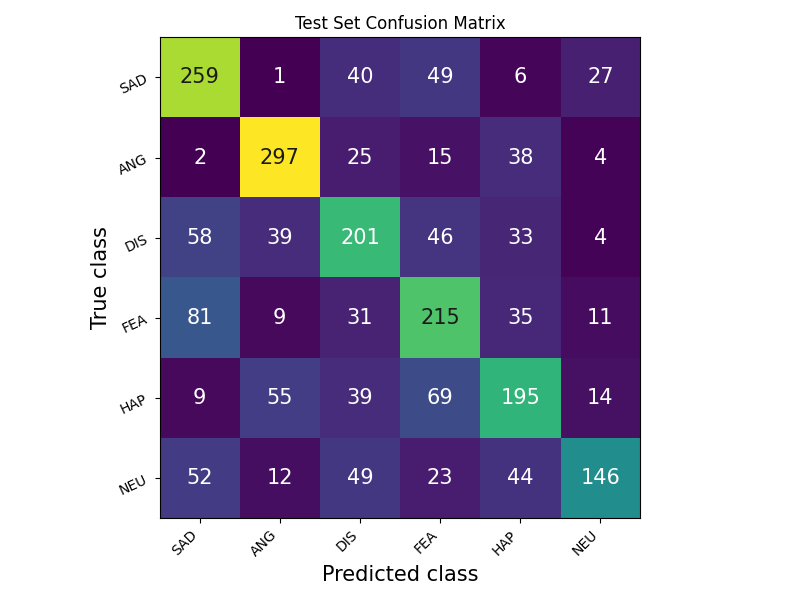
\includegraphics[width=\textwidth]{1D/lr0.001-ELU-1D-CF.png}
        \caption{ELU, lr=0.001}
    \end{subfigure}
    \caption{Confusion matrices for 1D CNN models with learning rate 0.001 and different activation functions}
    \label{fig:1d_confusion_matrices}
\end{figure}

\subsubsection{2D CNN Model Confusion Matrices}

\begin{figure}[h]
    \centering
    \begin{subfigure}[b]{0.32\textwidth}
        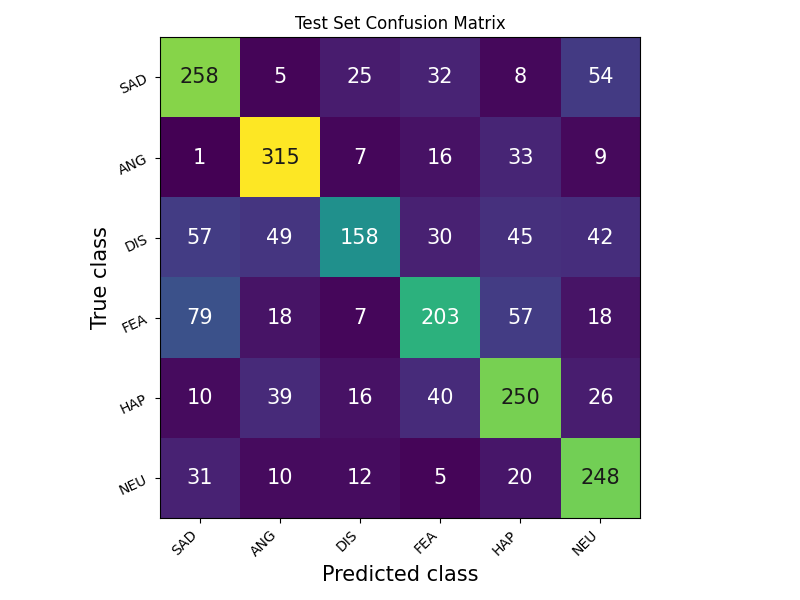
\includegraphics[width=\textwidth]{2D/lr0.001-SiLU-2D-CF.png}
        \caption{SiLU, lr=0.001}
    \end{subfigure}
    \begin{subfigure}[b]{0.32\textwidth}
        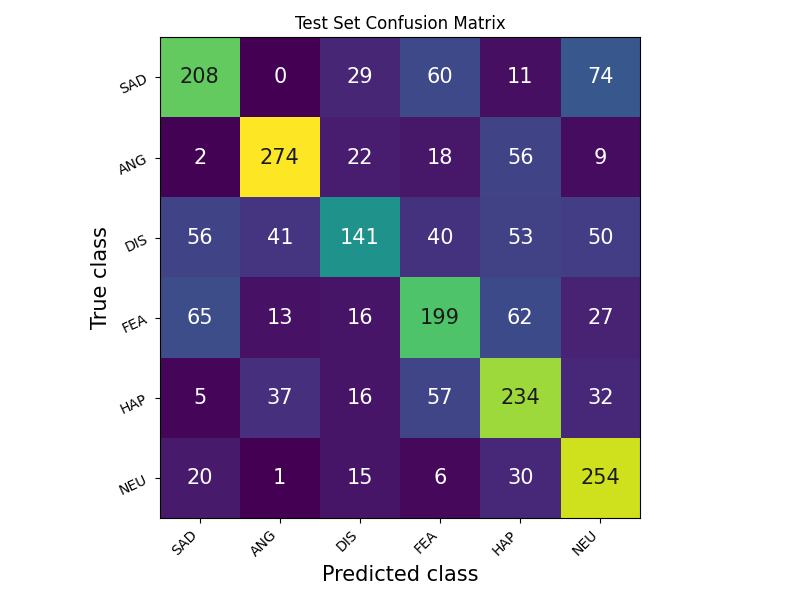
\includegraphics[width=\textwidth]{2D/lr0.001-ReLU-2D-CF.png}
        \caption{ReLU, lr=0.001}
    \end{subfigure}
    \begin{subfigure}[b]{0.32\textwidth}
        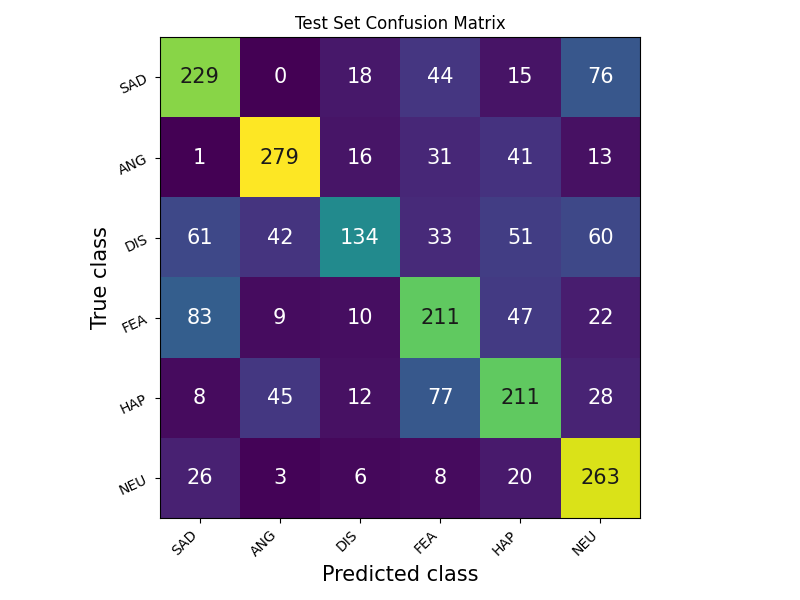
\includegraphics[width=\textwidth]{2D/lr0.001-ELU-2D-CF.png}
        \caption{ELU, lr=0.001}
    \end{subfigure}
    \caption{Confusion matrices for 2D CNN models with learning rate 0.001 and different activation functions}
    \label{fig:2d_confusion_matrices}
\end{figure}

The confusion matrices reveal several interesting patterns:

\begin{itemize}
    \item \textbf{Well-recognized emotions}: Anger (ANG) and Happiness (HAP) were the most accurately recognized emotions, with F1-scores of 0.76 and 0.71 respectively. These emotions typically involve more energetic speech patterns with distinctive acoustic features.
    
    \item \textbf{Confusing emotion pairs}: The most common confusions were between:
    \begin{itemize}
        \item Fear (FEA) and Sadness (SAD): These emotions share lower energy and similar pitch patterns
        \item Disgust (DIS) and Anger (ANG): Both can involve tense vocal expressions
        \item Neutral (NEU) and Sadness (SAD): Subtle expressions of sadness can be mistaken for neutral speech
    \end{itemize}
    
    \item \textbf{Challenging emotion}: Fear (FEA) was the most challenging emotion to recognize, with the lowest class-specific F1-score of 0.55. It was frequently confused with both Sadness and Disgust.
\end{itemize}

These patterns align with findings in the literature that suggest acoustically similar emotions are harder to distinguish in SER systems.

\subsection{Training and Validation Performance}

\begin{figure}[h]
    \centering
    \begin{subfigure}[b]{0.48\textwidth}
        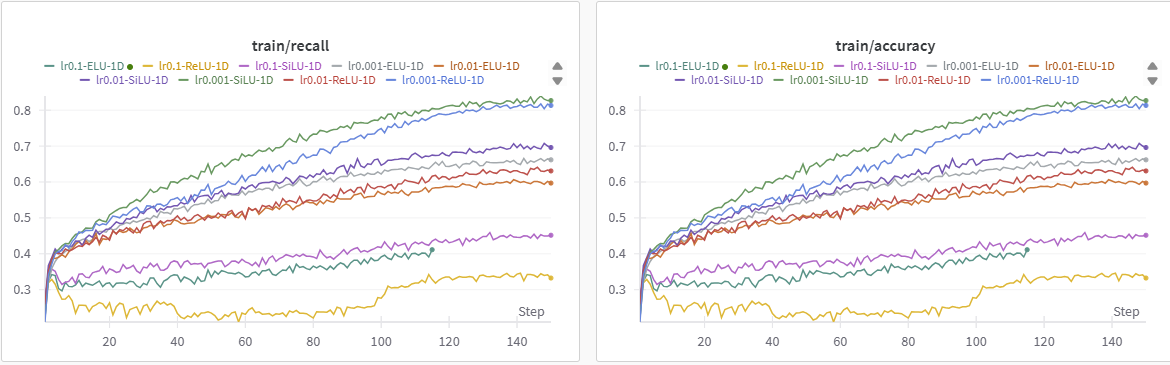
\includegraphics[width=\textwidth]{1D/1d-train.png}
        \caption{1D CNN Training Curves}
    \end{subfigure}
    \hfill
    \begin{subfigure}[b]{0.48\textwidth}
        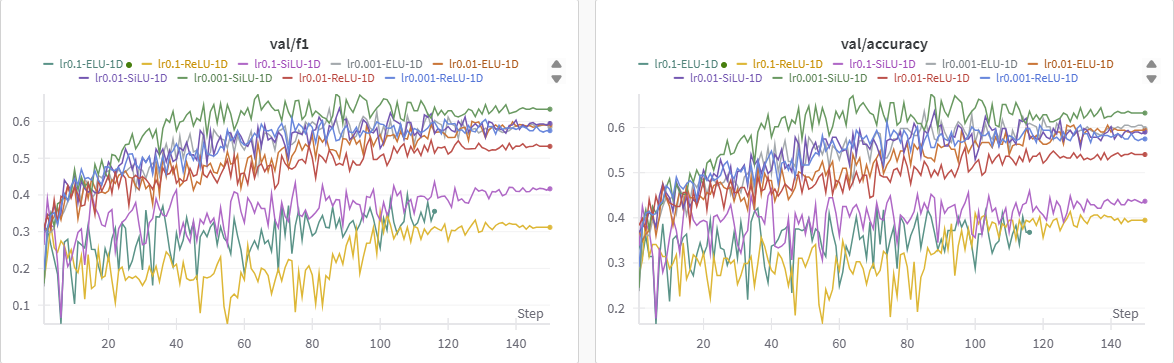
\includegraphics[width=\textwidth]{1D/1d-val.png}
        \caption{1D CNN Validation Curves}
    \end{subfigure}
    \caption{Training and validation performance curves for 1D CNN models}
    \label{fig:1d_training_curves}
\end{figure}

\begin{figure}[h]
    \centering
    \begin{subfigure}[b]{0.48\textwidth}
        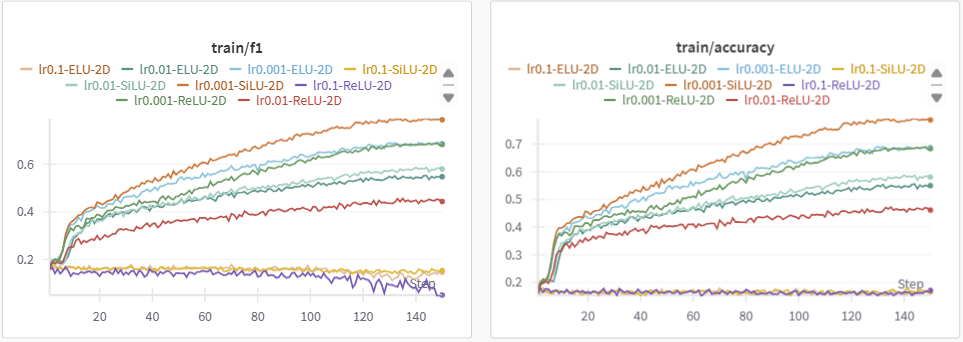
\includegraphics[width=\textwidth]{2D/2d-train.png}
        \caption{2D CNN Training Curves}
    \end{subfigure}
    \hfill
    \begin{subfigure}[b]{0.48\textwidth}
        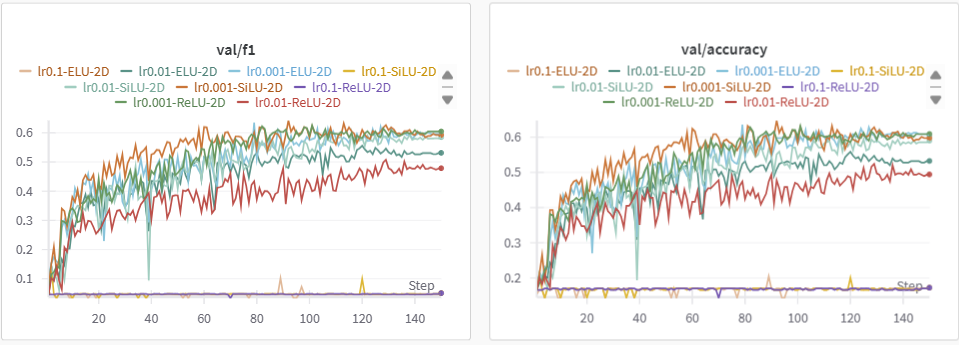
\includegraphics[width=\textwidth]{2D/2d-val.png}
        \caption{2D CNN Validation Curves}
    \end{subfigure}
    \caption{Training and validation performance curves for 2D CNN models}
    \label{fig:2d_training_curves}
\end{figure}

The 2D CNN with SiLU activation converged more quickly and achieved better validation loss than the other models. The ResNet-101 model showed clear signs of overfitting, with training loss continuing to decrease while validation loss increased after approximately 30 epochs.

\subsection{Architecture Modifications}

We also experimented with architectural modifications to understand their impact on model performance:

\begin{itemize}
    \item \textbf{Variable length input}: Processing audio with its original variable length rather than fixed-size inputs improved the combined model's performance from 61.3\% to 62.2\% accuracy. This suggests that preserving temporal dynamics across different audio samples provides useful information for emotion recognition.
    
    \item \textbf{Fixed 2D input dimensions}: Standardizing the mel spectrogram to exactly 64×64 pixels provided a good balance between preserving relevant information and computational efficiency.
    
    \item \textbf{Single-channel 1D features}: Using mean aggregation over time to create fixed-size 1D features achieved reasonable accuracy while significantly reducing the model size and training time.
    
    \item \textbf{ResNet architectures}: Despite their success in image classification, both ResNet-38 and ResNet-101 showed poor performance for SER. ResNet-101 exhibited severe overfitting (training accuracy of 70\% vs. validation accuracy of 41\%), suggesting that the architecture was too complex for the size of our dataset.
\end{itemize}

\subsection{Discussion}

Our experiments demonstrated that:

\begin{enumerate}
    \item \textbf{2D representations are powerful}: The 2D CNN with mel spectrogram inputs outperformed other approaches, reaching 64.1\% accuracy with SiLU activation, highlighting the importance of spectral-temporal patterns in emotion recognition.
    
    \item \textbf{Advanced activation functions matter}: SiLU (Swish) activation function significantly improved performance, particularly for 2D CNN models, offering almost 6\% absolute improvement over ReLU for the same architecture.
    
    \item \textbf{Variable length processing is beneficial}: Preserving the original temporal structure of audio improved results compared to fixed-size processing, confirming that emotion expression timing patterns are important.
    
    \item \textbf{Learning rate tuning is critical}: The optimal learning rate varied across architectures, with 0.001 being optimal for 2D and combined models while 0.01 worked better for 1D CNNs.
    
    \item \textbf{Some emotions are inherently harder to distinguish}: Emotions with similar acoustic characteristics (e.g., Fear and Sadness) remain challenging to differentiate, suggesting that additional contextual or linguistic features might be necessary to improve performance further.

    \item \textbf{Model complexity requires sufficient data}: More complex models like ResNet-101 performed worse due to overfitting, indicating that the dataset size is a limiting factor.
\end{enumerate}

These findings align with recent research in SER, which increasingly emphasizes the importance of appropriate feature representation, activation function selection, and careful hyperparameter tuning for optimal performance.